\chapter{Experimental Results}
\label{ch:experimental}
\begin{figure}[h]
    \centering
    \begin{minipage}{0.9\textwidth}
        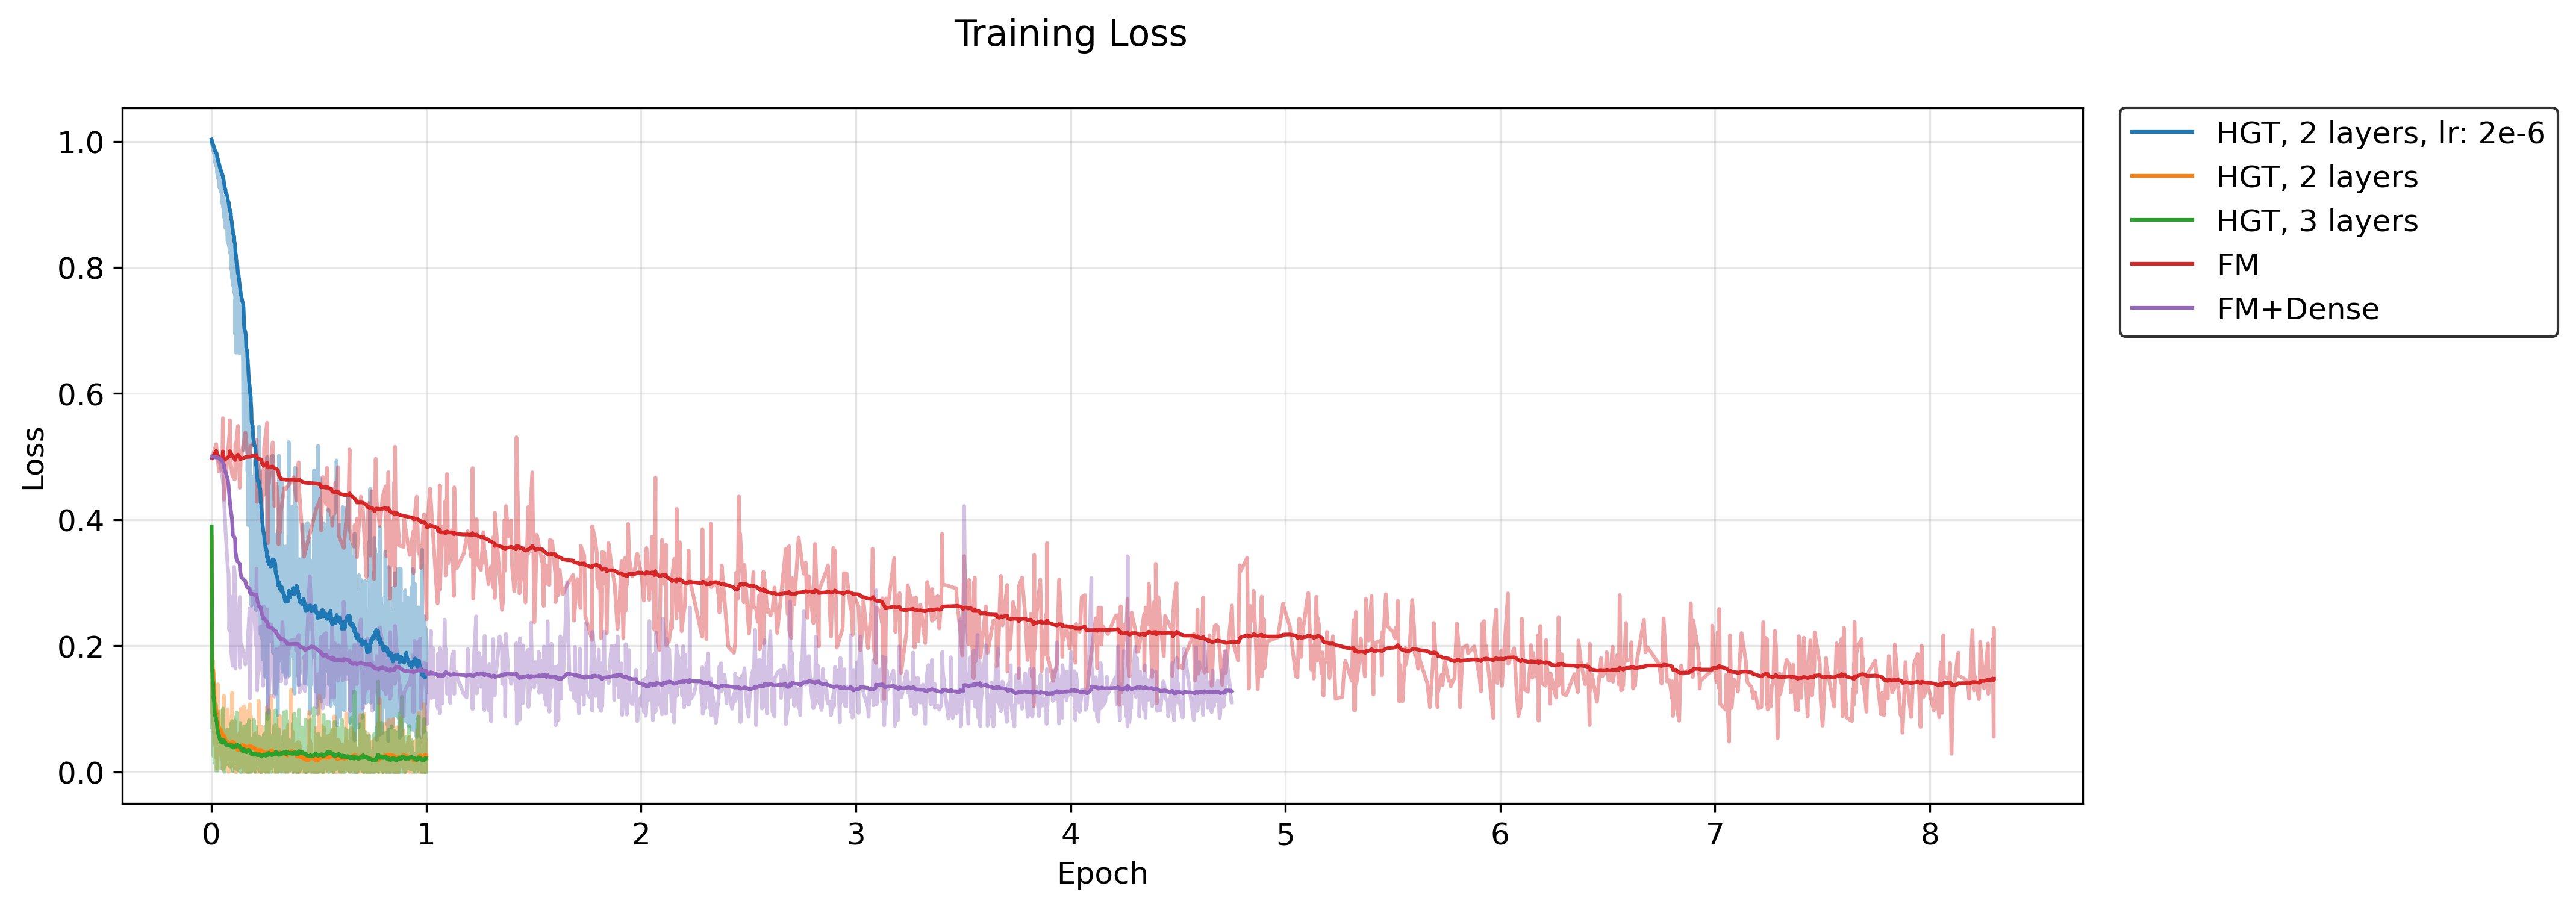
\includegraphics[width=\textwidth]{img/trainloss.png}
       
    \end{minipage}
    
    \begin{minipage}{0.9\textwidth}
        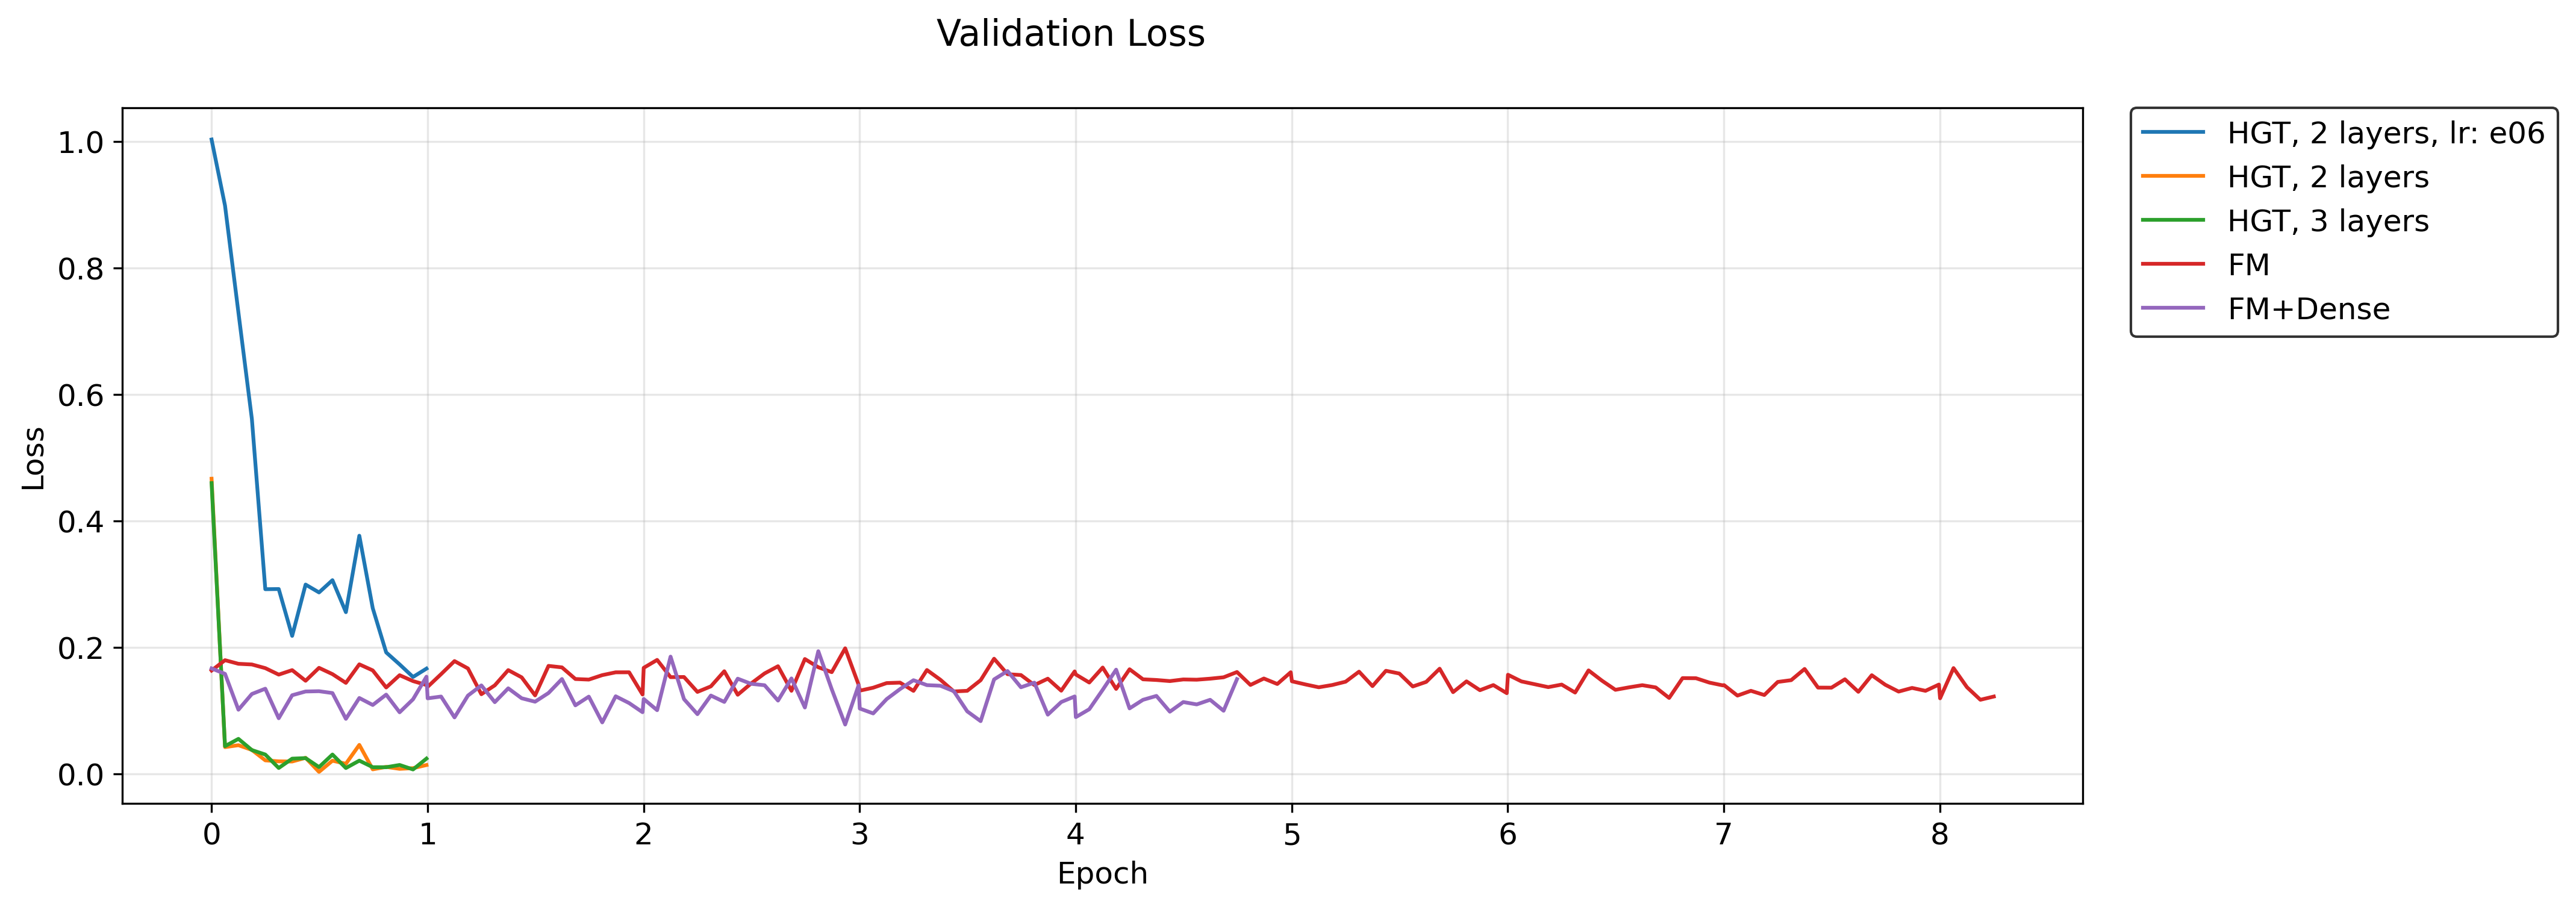
\includegraphics[width=\textwidth]{img/valloss.png}
       
    \end{minipage}
        \caption{Training and validation loss of the baselines and GNN-based systems}
     \label{fig:valloss}
\end{figure}

Each of the GNN-based systems is trained for one epoch only due to computational constraints. The duration of training one epoch on the NVIDIA Tesla T4 GPU is five hours. The baseline systems are trained for additional epochs until their loss converges on the training set, as no large loss decrease on the validation set is visible. Later, the second baseline is trained for further 59 epochs to ensure that the validation loss does not decrease visibly beyond the point depicted in Figure \ref{fig:valloss}. 

Training the baselines for more epochs is required for a fair comparison as the GNN has technically seen more data during one epoch, the node features of the whole subgraph, whereas the baselines only see the categorical, handcrafted and averaged features. The training loss on the mini-batches is smoothed for better comparability, and the real values are provided in faded colors. Validation loss is not computed on the whole validation set but mini-batches only, for performance reasons. The models' complexity is not comparable by parameter count, as the FM will only use a small subset of parameters for the categorical features during computation and the GNN-based systems active parameter count is dependent on the sampled subgraph. For reference, the second baseline has $350\cdot10^6$ trainable parameters, the three-layer HGT $\,5\cdot10^6$ trainable parameters.

The HGT with the worst performance, the learning rate of $2\cdot10^{-6}$ is included as reference as the validation loss is comparable to the loss of the baselines, and could surpass their loss as indicated by the curve of the training loss. The four-layer HGT performs similar to the other depicted HGTs, hence it is not included in the evaluation. The baseline which includes the continuous numerical features has in tendency slightly lower validation loss than the FM. The final validation losses on the mini-batches are 0.166, 0.150, 0.122, 0.024 and 0.014 respectively.




\begin{table}
\centering

\begin{tabular}{|c|c|c|c|c|c|}
\hline
Split: & \multicolumn{2}{c|}{Train} & \multicolumn{2}{c|}{Test} \\
 \hline
  & MRR & Mean Rank & MRR & Mean Rank \\
\hline
FM &  0.024 $\pm$0.073 & 5374 $\pm$ 11418& 0.014 $\pm$ 0.104 & 7749 $\pm$ 12796 \\
\hline
FM+NN & 0.075  $\pm$  0.183&2799 $\pm$ 6843& 0.074 $\pm$ 0.179 & 2981 $\pm$ 7207 \\
\hline
HGT, 2 layers & 0.380 $\pm$ 0.440 &  1122 $\pm$ 5193 & 0.368 $\pm$ 0.449 & \textbf{880.5} $\pm$ 3741 \\
\hline
HGT, 3 layers &  0.484 $\pm$ 0.478 & 1956 $\pm$ 5052 & \textbf{0.524} $\pm$ 0.487  &  1776 $\pm$ 4179  \\  \hline
\end{tabular}
\caption{Final MRR and mean rank}
\label{tab:finalscores}

\end{table}


Table \ref{tab:finalscores} depicts the MRR and mean rank obtained on all target edges from the train and test set. The rank of the positive edge is tested against all 55,000 negative edges to other courses. The three-layer HGT outperforms the best factorization based solution by 0.450 in MRR on the test set. Still, the three-layer HGTs' test MRR has a large sample standard deviation of 0.487. The addition of the continuous numerical features to the baseline improves test-MRR by 0.06. Interestingly, the two-layer HGT has a better mean rank than the three-layer HGT. The results are further discussed in the next chapter. Surprisingly, the MRR of the three-layer HGT and the mean ranks of both HGTs on the test set are better than on the training set. This is attributed to the larger training supervision-set size of 27.75\% compared to the test set size of 5\%.  


\begin{table}[h]
\centering

\begin{tabular}{|c|c|c|}
\hline
Edge Type & Train & Test \\
 \hline
  & MRR & MRR\\
  \hline
Mean &  0.090 & 0.080   \\
\hline
skill→job & 0.128 & 0.094  \\
\hline
skill→qualification &0.067 & 0.077  \\
\hline
skill→skill & 0.126 &0.064 \\
\hline
job→job &0.122 & 0.131\\
\hline
job→person & 0.065 &0.074 \\
\hline
skill→course & 0.059 &0.062 \\
\hline
course→person & 0.108 &0.063 \\
\hline
course→qualification & 0.105 &0.074 \\
\hline
job→broader job & 0.046 &0.083 \\
\hline
person→organization & 0.103 &0.088  \\
\hline
person→supervisor & 0.053 &0.066 \\
\hline

\end{tabular}
\caption[General link prediction scores]{General link prediction scores, computed on a subset only}
\label{tab:finalscoresgeneral}

\end{table}

Notably, for the computation of the test scores of the GNN, the same sampling implementation as during training is utilized. Perhaps even better scores can be obtained by computing node embeddings multiple times on differently sampled subgraphs and by averaging the results. A qualitative example of content recommended by the three-layer HGT is provided in the Appendix \ref{ch:recommendedcontent}.



Table \ref{tab:finalscoresgeneral} shows the results of the general link prediction. Scores are only approximate, as they are computed on only 1000 edges per split. 